\section{Теорема об инкрементальной компиляции}

Рассмотрим ситуацию, когда для некоторого состояния проекта, представляемого набором исходных файлов, была проведена успешная полная компиляция в пустом контексте, то есть не использующая ничего, кроме самих исходных файлов; результат этой компиляции был сохранён в некотором кэше; затем разработчик удалил, добавил или изменил некоторые файлы, модифицировав таким образом состояние проекта; затем он собирается скомпилировать это новое состояние. Разумеется, он может провести повторную полную компиляцию нового состояния в пустом контексте. Однако можно воспользоваться тем, что результат повторной компиляции файлов, которые не подверглись изменению и не зависели существенным образом от изменившихся, будет совпадать с результатом первой компиляции. Это значит, что для этих файлов можно взять результат компиляции из кэша, а остальные подвергнуть перекомпиляции, сэкономив таким образом вычислительные ресурсы. Это интуитивное умозаключение формализуется в теореме об инкрементальной компиляции.\\

\newcommand{\butpartial}{{\sigma\setminus\rho\setminus\partial_1}}
\newcommand{\butpartialA}{{\alpha\setminus{\partial_2}}}
\newcommand{\sigmanoro}{{\sigma\setminus\rho}}

\textbf{Теорема 1 (об инкрементальной компиляции).}

Пусть дано: $\sigma \subset \Sigma$, $gen(\varnothing, \sigma) = \omega^\sigma$.
Пусть $\rho, \alpha \subset \Sigma$, при этом $\rho \subseteq \sigma$, $\sigma \cap \alpha = \varnothing$; $\Delta = \Delta^\rho_\alpha\sigma = \sigma\setminus\rho\cup\alpha$.
Известно, что определено $gen(\omega^\sigma_{\sigma\setminus\rho}, \alpha) = \omega_\alpha$ и $gen(\varnothing, \Delta) = \omega^\Delta$.
Обозначим 
$$\partial_1 = \partial\dfrac{\omega^\sigma_\rho}{\omega_\alpha}(\sigma\setminus\rho),$$
$$\omega^1_{\partial_1} = gen(\omega^\sigma_{\butpartial} \cup \omega_\alpha, \partial_1),$$
$$\partial_2 = \partial\dfrac{\omega^\sigma_{\sigma\setminus\rho}}{\omega^\sigma_{\butpartial} \cup \omega^1_{\partial_1}}(\alpha),$$
$$\omega^2_{\partial_2} = gen(\omega^\sigma_{\butpartial} \cup \omega_{\butpartialA} \cup \omega^1_{\partial_1}, \partial_2).$$
Тогда:

$$gen(\varnothing, \Delta) =^2 \omega^\sigma_{\butpartial} \cup \omega_{\butpartialA} \cup \omega^1_{\partial_1} \cup \omega^2_{\partial_2}$$

Здесь состояниям проекта соответствуют наборы входов функции компиляции; изменению файлов, содержащихся в проекте, соответствует вычитание из набора входов одного множества и добавление другого. Исходное состояние проекта обозначено $\sigma$, из него удаляются файлы множества $\rho$ и добавляются файлы множества $\alpha$. Тогда получившееся новое состояние являет собой $\sigma\setminus\rho\cup\alpha$. Внутри множества $\sigma\setminus\rho$ выделяется дифференциал $\partial_1$, а внутри множества $\alpha$~--- дифференциал $\partial_2$. Файлы, соответствующие множествам дифференциалов, перекомпилируются в указанном в теореме контексте. Проиллюстрируем происходящее. На рис.~\ref{fig:theorem1_src} показаны рассматриваемые множества входов и их подмножества, на рис.~\ref{fig:theorem1_dst}~--- соответствующие им порождения. После объединения результата компиляции $\alpha$ и кэша для $\sigma\setminus\rho$ совпадение с результатом полной сборки будет иметь место только до нулевого порядка. После компиляции $\partial_1$ и объединения с соответствующим результатом получится совпадение до первого порядка. После компиляции $\partial_2$ и объединения с соответствующим результатом получится совпадение до второго порядка.

\begin{figure}[h!]
	\centering
	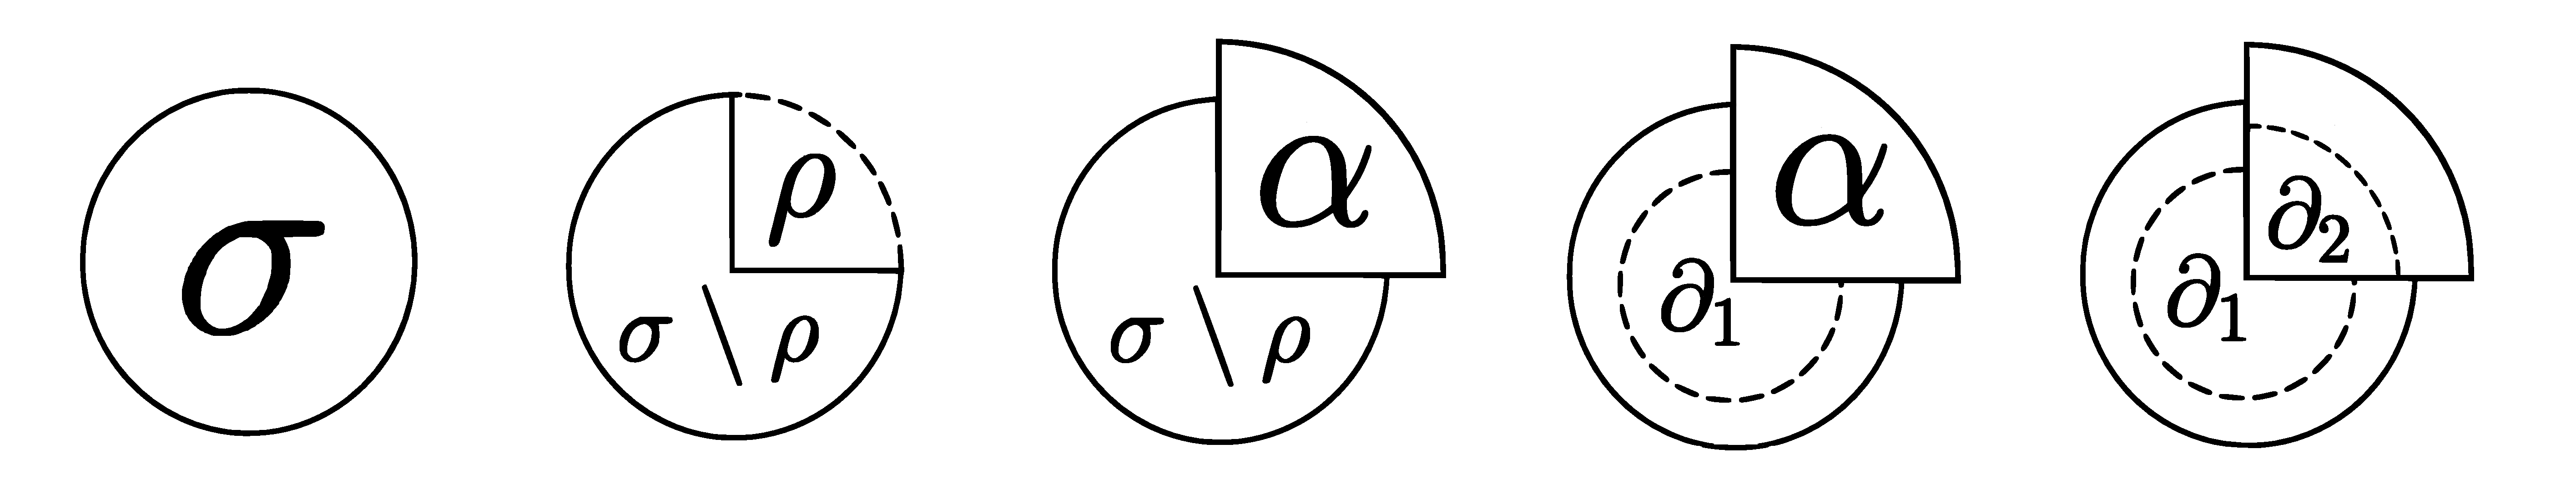
\includegraphics[width=11cm]{theorem1_src.eps}
	\caption{Рассматриваемые в теореме 1 множества входов и их подмножества}
	\label{fig:theorem1_src}
\end{figure}

\begin{figure}[h!]
	\centering
	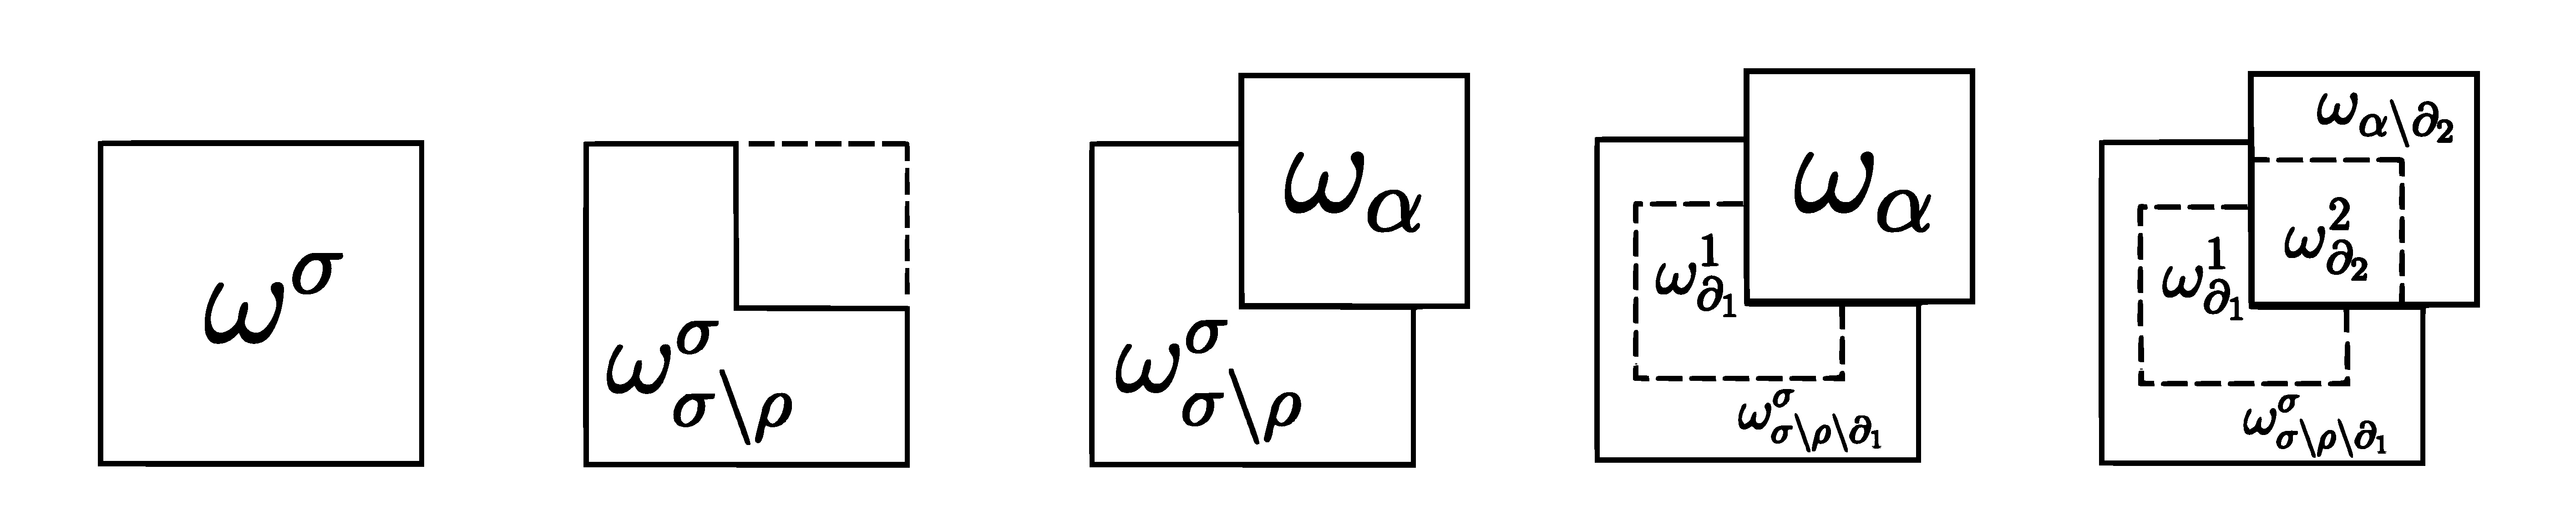
\includegraphics[width=11cm]{theorem1_dst.eps}
	\caption{Порождения, соответствующие множествам и подмножествам входов}
	\label{fig:theorem1_dst}
\end{figure}

Практическое применение данной теоремы таково: в ситуации, когда сохранён кэш для некоторого состояния проекта, которое впоследствии было изменено, предлагается обоснование подхода, состоящего в переиспользовании кэша и перекомпилировании меньшего количества файлов и, таким образом, позволяющего избежать полной компиляции этого состояния; предъявляется множество файлов, для которых следует переиспользовать кэш, множество файлов, которые следует перекомпилировать, а также контекст, в котором нужно проводить компиляцию, чтобы получившийся результат совпал с результатом полной компиляции нового состояния в пустом контексте.

\textbf{Доказательство:}
Докажем сначала, что $gen(\varnothing, \Delta) =^0 \omega^\sigma_{\sigma\setminus\rho} \cup \omega_\alpha$. По аксиоме о дизъюнктном разбиении $gen(\varnothing, \Delta) = \omega^\Delta_\sigmanoro \cup \omega^\Delta_\alpha$. При этом по аксиоме об эквивалентных контекстах $\omega^\Delta_\sigmanoro =^0 \omega^\sigma_{\sigma\setminus\rho}$. Рассмотрим $$\omega^\Delta_\alpha = gen(\omega^\Delta_{\sigma\setminus\rho}, \alpha)$$ 
и $$\omega_\alpha = gen(\omega^\sigma_{\sigma\setminus\rho}, \alpha).$$ 
Поскольку $$\omega^\Delta_{\sigma\setminus\rho} =^0 \omega^\sigma_{\sigma\setminus\rho},$$ 
то по аксиоме об эквивалентных контекстах $$\omega^\Delta_\alpha =^1 \omega_\alpha.$$ Тогда, действительно, $$gen(\varnothing, \Delta) =^0 \omega^\sigma_{\sigma\setminus\rho} \cup \omega_\alpha.$$ 

Докажем, что дифференциал $\partial_1 = \partial\dfrac{\omega^\sigma_\rho}{\omega_\alpha}(\sigma\setminus\rho)$ имеет смысл. Для этого проверим, что определены $gen(\omega^\sigma_\rho, \sigma\setminus\rho)$ и $gen(\omega_\alpha, \sigma\setminus\rho)$. Первое выражение~--- это $\omega^\sigma_{\sigma\setminus\rho}$ и определено по аксиоме о дизъюнктном разбиении. Рассмотрим второе выражение: поскольку $\omega^\Delta_\alpha =^1 \omega_\alpha$ и $gen(\omega^\Delta_\alpha, \sigma\setminus\rho)$ определено, то и $gen(\omega_\alpha, \sigma\setminus\rho)$ определено. Тогда дифференциал, действительно, имеет смысл.

Докажем, что определено $\omega^1_{\partial_1}$. Поскольку определено $gen(\omega^\Delta_{\butpartial \cup \alpha}, \partial_1)$ и $\omega^\sigma_{\butpartial} \cup \omega_\alpha =^0 \omega^\Delta_{\butpartial \cup \alpha}$, то по аксиоме об эквивалентных контекстах $\omega^1_{\partial_1} = gen(\omega^\sigma_{\butpartial} \cup \omega_\alpha, \partial_1)$ определено.

Докажем теперь, что $$gen(\varnothing, \Delta) =^1 \omega^\sigma_{\butpartial} \cup \omega_\alpha \cup \omega^1_{\partial_1}.$$ 
По аксиоме о дизъюнктном разбиении $$gen(\varnothing, \Delta) = \omega^\Delta_\butpartial \cup \omega^\Delta_\alpha \cup \omega^\Delta_{\partial_1}.$$ 
Уже доказано, что $\omega^\Delta_\alpha =^1 \omega_\alpha$. По лемме об эквивалентном дифференциале $$gen(\omega^\sigma_\rho \cup \omega^\sigma_{\partial_1}, \butpartial) =^2 gen(\omega^\Delta_\alpha \cup \omega^\Delta_{\partial_1}, \butpartial),$$ 
то есть $\omega^\sigma_{\butpartial} =^2 \omega^\Delta_{\butpartial}$. Таким образом, $$\omega^\Delta_\butpartial \cup \omega^\Delta_\alpha =^1 \omega^\sigma_{\butpartial} \cup \omega_\alpha.$$ 
Поэтому $$\omega^\Delta_{\partial_1} = gen(\omega^\Delta_\butpartial \cup \omega^\Delta_\alpha, \partial_1) =^2 gen(\omega^\sigma_{\butpartial} \cup \omega_\alpha, \partial_1) = \omega^1_{\partial_1}.$$ Тогда, действительно, выполняется равенство с точностью до первого порядка.

Докажем, что дифференциал $$\partial_2 = \partial\dfrac{\omega^\sigma_{\sigma\setminus\rho}}{\omega^\sigma_{\butpartial} \cup \omega^1_{\partial_1}}(\alpha)$$ 
имеет смысл. Для этого проверим, что определены $gen(\omega^\sigma_{\sigma\setminus\rho}, \alpha)$ и $gen(\omega^\sigma_{\butpartial} \cup \omega^1_{\partial_1}, \alpha)$. Первое выражение~--- это $\omega_\alpha$, оно определено по условию. Рассмотрим второе выражение: поскольку $$\omega^\sigma_{\butpartial} \cup \omega^1_{\partial_1} =^0 \omega^\Delta_{\sigmanoro}$$ 
и $gen(\omega^\Delta_{\sigmanoro}, \alpha)$ определено, то и $gen(\omega^\sigma_{\butpartial} \cup \omega^1_{\partial_1}, \alpha)$ определено. Тогда дифференциал, действительно, имеет смысл.

Докажем, что определено $\omega^2_{\partial_2}$. Поскольку определено $gen(\omega^\Delta_{\sigmanoro \cup \butpartialA}, \partial_2)$ и $$\omega^\sigma_{\butpartial} \cup \omega_{\butpartialA} \cup \omega^1_{\partial_1} =^0 \omega^\Delta_{\sigmanoro \cup \butpartialA},$$ то по аксиоме об эквивалентных контекстах $$\omega^2_{\partial_2} = gen(\omega^\sigma_{\butpartial} \cup \omega_{\butpartialA} \cup \omega^1_{\partial_1}, \partial_2)$$ 
определено.

Докажем теперь, что $$gen(\varnothing, \Delta) =^2 \omega^\sigma_{\butpartial} \cup \omega_{\butpartialA} \cup \omega^1_{\partial_1} \cup \omega^2_{\partial_2}.$$ 
По аксиоме о дизъюнктном разбиении $$gen(\varnothing, \Delta) = \omega^\Delta_\butpartial \cup \omega^\Delta_\butpartialA \cup \omega^\Delta_{\partial_1} \cup \omega^\Delta_{\partial_2}.$$ 
Уже доказано, что $\omega^\Delta_{\butpartial} =^2 \omega^\sigma_{\butpartial}$, $\omega^\Delta_{\partial_1} =^2 \omega^1_{\partial_1}$. Из этого следует, что $\omega^\Delta_{\sigmanoro} =^2 \omega^\sigma_{\butpartial} \cup \omega^1_{\partial_1}$. По лемме об эквивалентном дифференциале $$gen(\omega^\sigma_{\sigmanoro} \cup \omega^\alpha_{\partial_2}, \butpartialA) =^3 gen(\omega^\Delta_\sigmanoro \cup \omega^\Delta_{\partial_2}, \butpartialA),$$ 
то есть $\omega_{\butpartialA} =^3 \omega^\Delta_{\butpartialA}$. Таким образом, $$\omega^\Delta_{\sigmanoro} \cup \omega^\Delta_{\butpartialA} =^2 \omega^\sigma_{\butpartial} \cup \omega_{\butpartialA} \cup \omega^1_{\partial_1}.$$ 
Поэтому $$\omega^\Delta_{\partial_2} = gen(\omega^\Delta_{\sigmanoro} \cup \omega^\Delta_{\butpartialA}, \partial_2) =^3 gen(\omega^\sigma_{\butpartial} \cup \omega_{\butpartialA} \cup \omega^1_{\partial_1}, \partial_2) = \omega^2_{\partial_2}.$$ 
Тогда, действительно, выполняется равенство с точностью до второго порядка. $\Box$\\
 
% ------------------------------------------------------
\newpage
\section{Теорема о переиспользовании порождений}

Рассмотрим ситуацию, когда несколько разработчиков одновременно работают над одним и тем же проектом. Каждый разработчик редактирует файлы, составляющие его локальную копию проекта, и время от времени инкрементально собирает свою копию на своём же компьютере; таким образом, у каждого разработчика есть локальный кэш компиляции, в котором хранятся результаты последнего сеанса сборки. При условии регулярного обмена изменениями файлов, например, обновления локальных копий проекта из общего репозитория, можно предполагать, что эти локальные копии отличаются друг от друга незначительно. В процессе такой коллективной разработки случаются ситуации, когда состояние проекта в локальной копии разработчика существенно отличается от состояния, для которого был посчитан его локальный кэш компиляции. Тогда инкрементальная компиляция теряет свои преимущества и мало чем отличается от процедуры полной сборки проекта с нуля. Примерами таких случаев могут служить ``cold start''~--- сборка проекта в ситуации отсутствия кэша вообще~--- или переключение между ветками (``branches'')~--- например, основной и релизной ветками. В таких ситуациях может быть разумным при компиляции использовать вместо локального кэша компиляции кэши других разработчиков. Пусть у разработчика такое состояние проекта, что в целом виде оно не совпадает ни с одним из состояний других разработчиков, однако представимо в виде дизъюнктного объединения частей, каждая из которых присутствует у какого-либо другого разработчика. Тогда можно переиспользовать те подмножества кэшей, которые соответствуют результатам компиляции этих частей. Эта задача формализуется и решается в теореме о переиспользовании порождений.\\

\textbf{Теорема 2 (о переиспользовании порождений).}

\newcommand{\sigi}{{\sigma_i}}
\newcommand{\sigk}{{\sigma_k}}
\newcommand{\sigpi}{{\sigma^\prime_i}}
\newcommand{\sigpj}{{\sigma^\prime_j}}
\newcommand{\sigpk}{{\sigma^\prime_k}}
\newcommand{\parti}{{\partial_i}}
\newcommand{\partj}{{\partial_j}}
\newcommand{\partk}{{\partial_k}}
\newcommand{\xii}{{\xi_i}}
\newcommand{\xij}{{\xi_j}}
\newcommand{\xik}{{\xi_k}}
\newcommand{\sms}{{\setminus}}
\newcommand{\alloth}{\bigcup\limits_{j \neq i}\omega^\prime_j}
\newcommand{\allothk}{\bigcup\limits_{j \neq k}\omega^\prime_j}
\newcommand{\allothD}{\bigcup\limits_{j \neq i}\omega^\Delta_{\sigpj}}
\newcommand{\rprt}{{\text{п.ч.}}}

Пусть $\forall i \in [1:n]$ дано: $\sigma_i$, $\omega_i = gen(\varnothing, \sigma_i)$, $\sigma_i^\prime \subseteq \sigma_i$ ($\sigma_i^\prime \cap \sigma_j^\prime = \varnothing$ при $i \neq j$). Обозначим $\omega_i^\prime = gen_i(\sigma_i^\prime)$. Обозначим 
$$\partial_i = \partial\dfrac{\omega_i \setminus \omega_i^\prime}{\bigcup\limits_{j \neq i} \omega_j^\prime} \sigma_i^\prime,$$
$$\omega_{\bigcup\limits_k \partk} = gen(\bigcup\limits_k \omega_{\sigpk\sms\partk}, \bigcup\limits_k \partk),$$
$$\xi_i = \partial\dfrac{\omega_{\sigi\sms\sigpi \cup \parti}}{\bigcup\limits_{j \neq i} \omega_{\sigpj\sms\partj} \cup \omega_{\bigcup\limits_k \partial_k}} \sigpi\sms\parti.$$
Тогда:
$$gen(\varnothing, \bigcup\limits_k \sigpk) =^2 \bigcup\limits_k \omega_{\sigpk\sms\partk\sms\xik} \cup \omega_{\bigcup\limits_k \partial_k} \cup gen(\bigcup\limits_k \omega_{\sigpk\sms\partk\sms\xik} \cup \omega_{\bigcup\limits_k \partial_k}, \bigcup\limits_k \xik)$$

Как и в предыдущей теореме, состояниям проекта соответствуют наборы входов функции компиляции. Рассматривается $n$ состояний, обозначенных $\sigma_i$, для каждого из которых известен (кэширован) результат его компиляции $\omega_i$. Новое состояние представляется как объединение непересекающихся частей имеющихся состояний, обозначенных $\sigma^\prime_i$. Для нахождения результата компиляции этого нового состояния переиспользуются части известных кэшей, обозначенные $\omega^\prime_i$, а также докомпилируется некоторое подмножество этого состояния, выраженное с помощью дифференциалов. Проиллюстрируем происходящее с помощью примера для $n = 4$. На рис.~\ref{fig:theorem2_src} показаны известные состояния и выделенные в них непересекающиеся части, на рис.~\ref{fig:theorem2_dst}~--- соответствующие им порождения, на рис.~\ref{fig:theorem2_srcn}~--- новое состояние и выделяемые в нём подмножества, на рис.~\ref{fig:theorem2_dstn}~--- соответствующие им порождения.

\begin{figure}[h!]
	\centering
	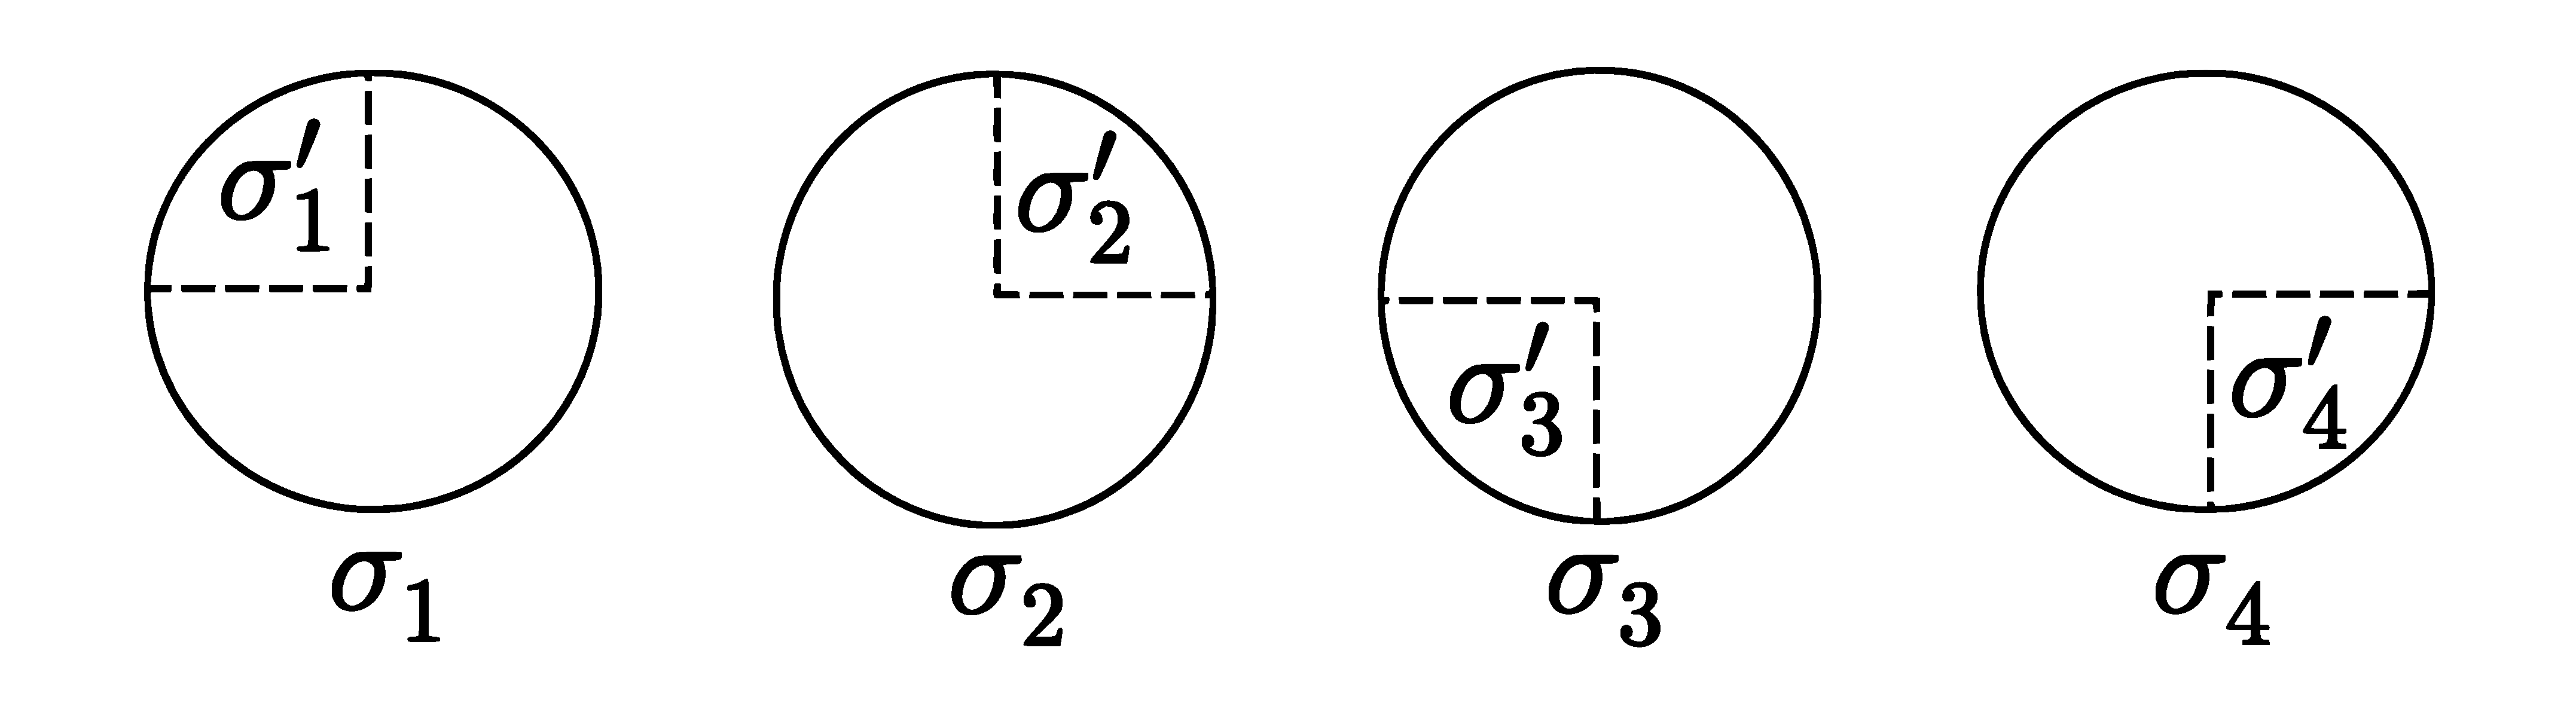
\includegraphics[width=11cm]{theorem2_src.eps}
	\caption{Рассматриваемые в теореме 2 известные состояния и выделенные в них части}
	\label{fig:theorem2_src}
\end{figure}

\begin{figure}[h!]
	\centering
	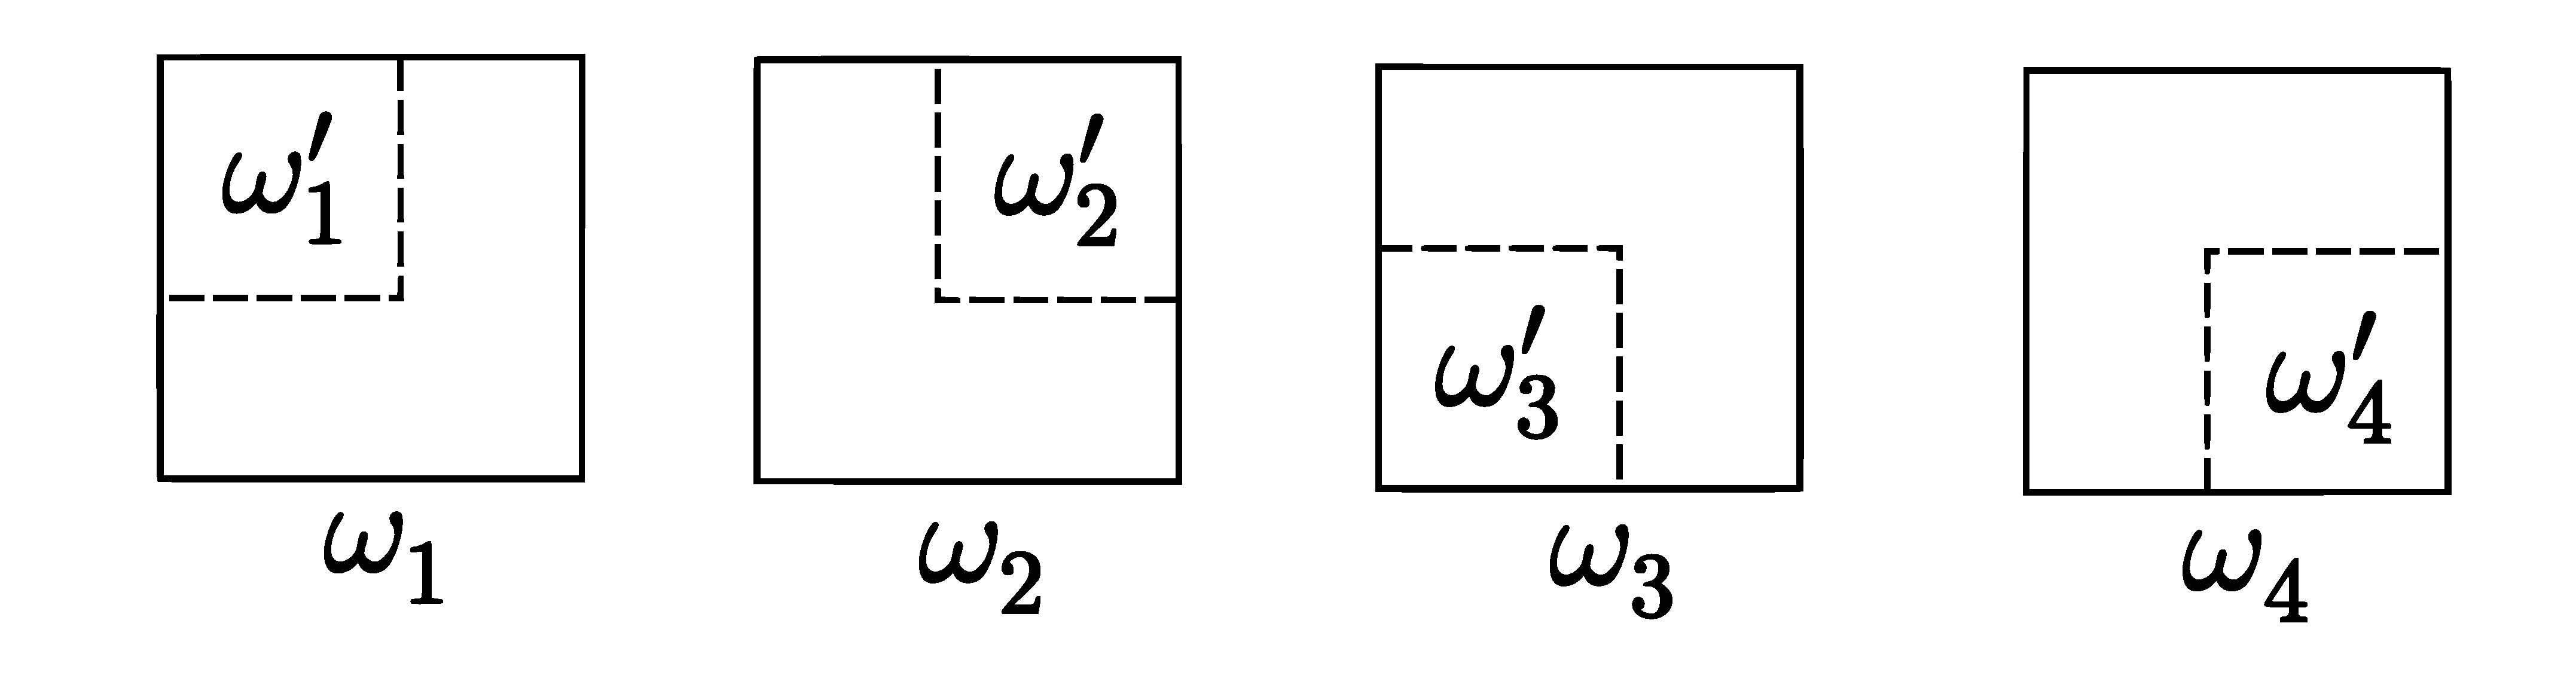
\includegraphics[width=11cm]{theorem2_dst.eps}
	\caption{Порождения, соответствующие известным состояниям и их частям}
	\label{fig:theorem2_dst}
\end{figure}

\begin{figure}[h!]
	\centering
	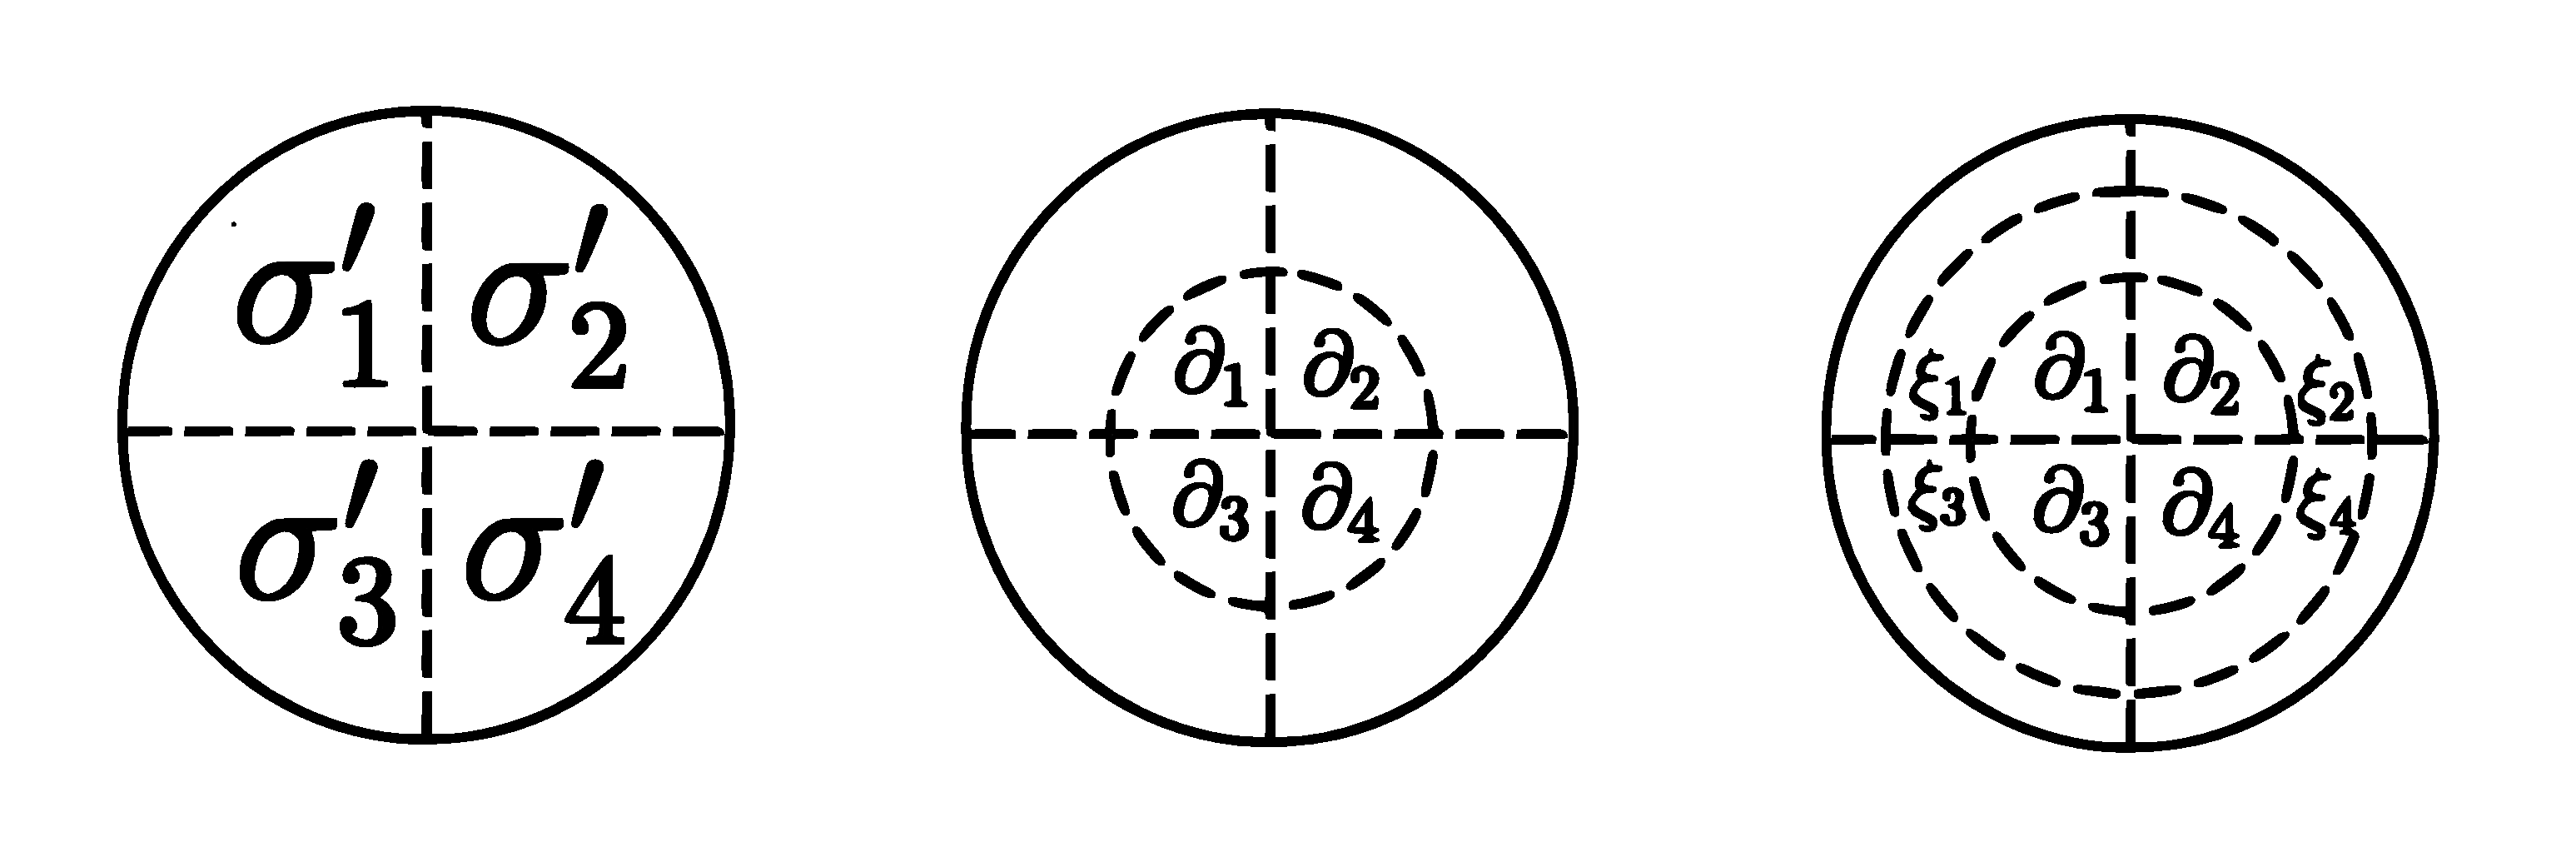
\includegraphics[width=11cm]{theorem2_srcn.eps}
	\caption{Рассматриваемое в теореме 2 новое состояние и выделяемые в нём подмножества}
	\label{fig:theorem2_srcn}
\end{figure}

\begin{figure}[h!]
	\centering
	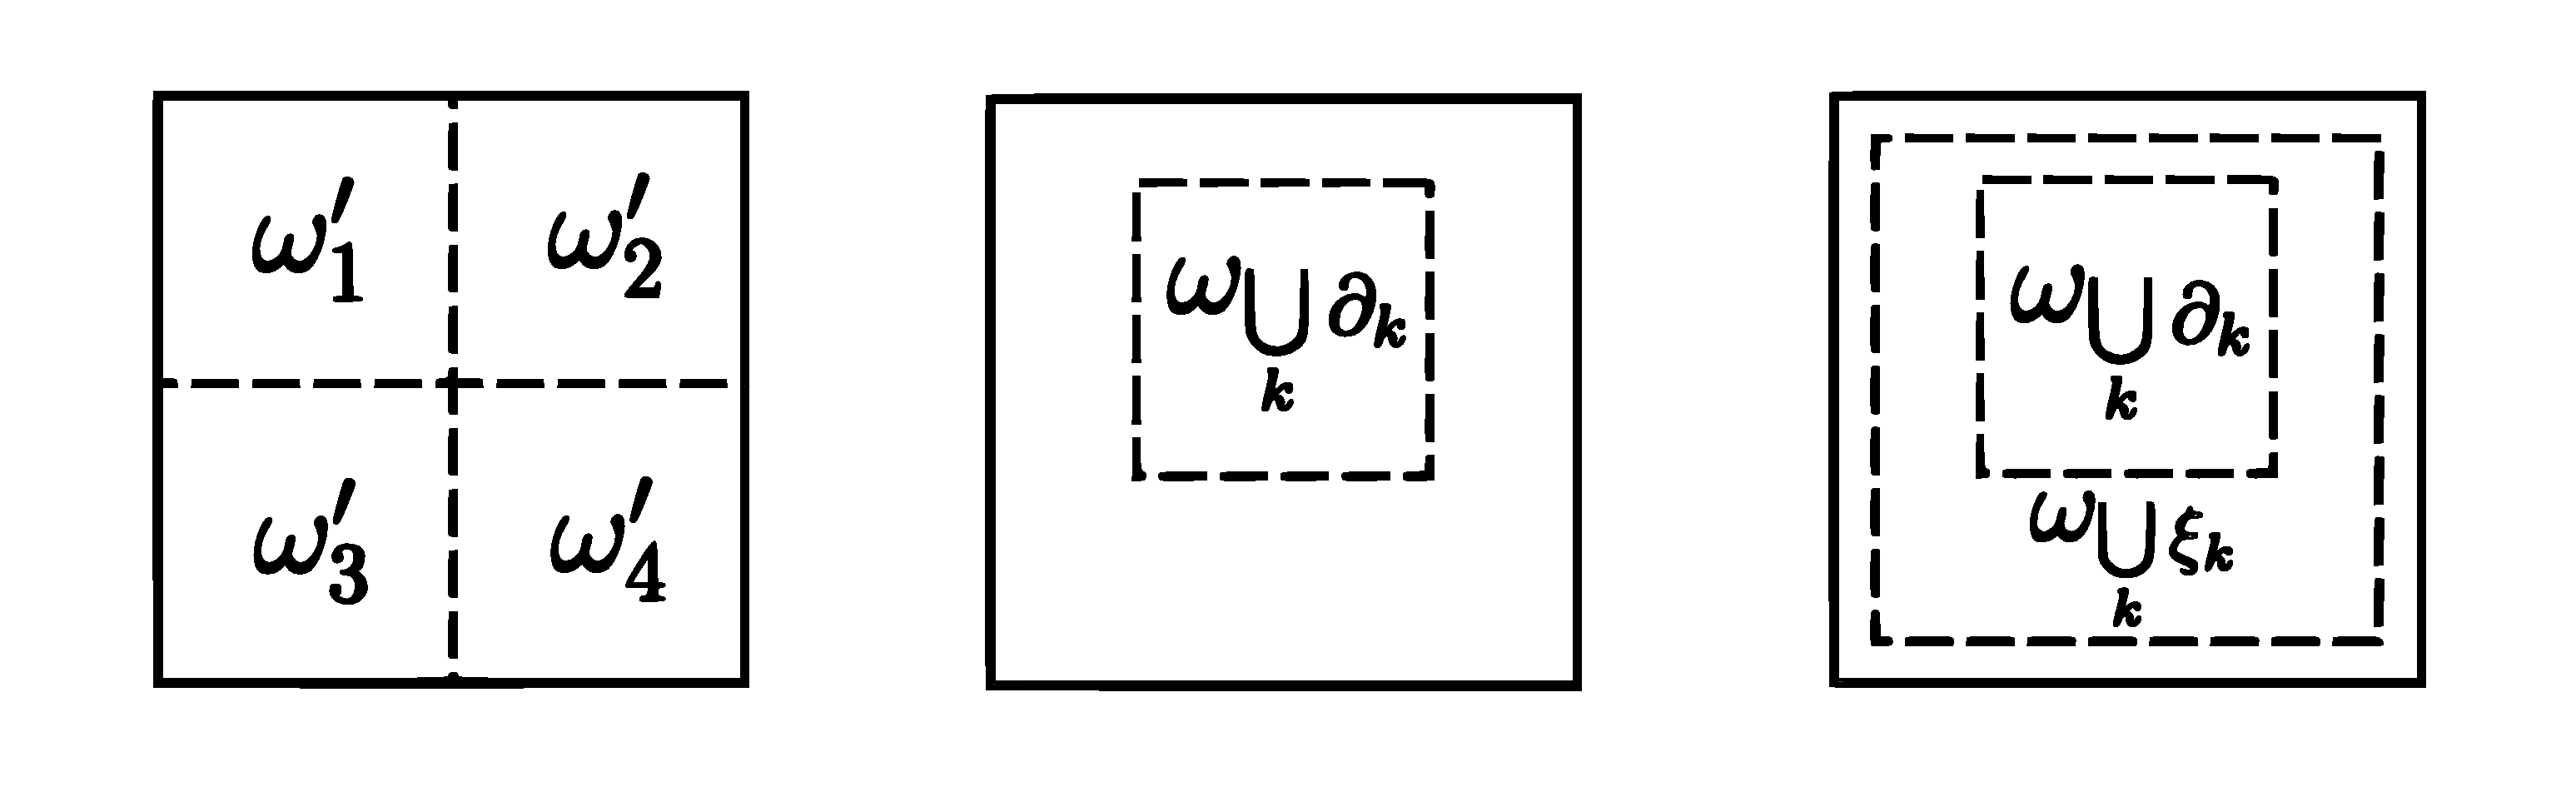
\includegraphics[width=11cm]{theorem2_dstn.eps}
	\caption{Порождения, соответствующие новому состоянию и его подмножествам}
	\label{fig:theorem2_dstn}
\end{figure}

Практическое применение данной теоремы таково: в ситуации, когда для некоторого состояния проекта неизвестен результат компиляции, но оно представимо в виде частей состояний с известными кэшированными результатами, предлагается подход, состоящий в переиспользовании части кэшей и перекомпилировании меньшего количества файлов и, таким образом, позволяющий избежать полной компиляции этого состояния; предъявляется множество файлов, для которых следует переиспользовать кэши, множество файлов, которые следует перекомпилировать, а также контекст, в котором нужно проводить компиляцию, чтобы получившийся результат совпал с результатом полной компиляции этого состояния в пустом контексте.

\textbf{Доказательство:}
Обозначим $\Delta = \bigcup\limits_k \sigpk$.

Докажем, что $$gen(\varnothing, \bigcup\limits_k \sigpk) =^0 \bigcup\limits_k \omega_{\sigpk}.$$ 
Для этого достаточно заметить, что $$gen(\varnothing, \bigcup\limits_k \sigpk) = \bigcup\limits_k \omega^\Delta_{\sigpk} =^0 \bigcup\limits_k \omega_{\sigpk}.$$

Докажем, что дифференциал $$\partial_i = \partial\dfrac{\omega_i \setminus \omega_i^\prime}{\alloth} \sigma_i^\prime$$ имеет смысл. Для этого проверим, что определены $gen(\omega_{\sigi} \setminus \omega_{\sigpi}, \sigpi)$ и $gen(\alloth, \sigpi)$. Поскольку определено $gen(\varnothing, \sigi)$, то по аксиоме о дизъюнктном разбиении определено и $gen(\omega_{\sigi} \setminus \omega_{\sigpi}, \sigpi)$. Далее, из определённости $gen(\varnothing, \bigcup\limits_k \sigma^\prime_k)$ по аксиоме о дизъюнктном разбиении следует определённость $gen(\bigcup\limits_{j \neq i}\omega^\Delta_\sigpj, \sigpi)$; поскольку $\bigcup\limits_{j \neq i}\omega^\Delta_\sigpj =^0 \alloth$, то отсюда по аксиоме об эквивалентных контекстах определено $gen(\alloth, \sigpi)$.

Докажем, что $$gen(\varnothing, \bigcup\limits_k \sigpk) =^1 \bigcup\limits_k \omega_{\sigpk\sms\partk} \cup gen(\bigcup\limits_k \omega_{\sigpk\sms\partk}, \bigcup\limits_k \partk).$$ 
По лемме об эквивалентном дифференциале для каждого $i$ из равенства $\allothD =^0 \bigcup\limits_{j \neq i} \omega_{\sigpj}$ следует $$gen(\omega_{\sigi\sms\sigpi} \cup \omega_\parti, \sigpi\sms\parti) =^1 gen(\allothD \cup \omega^\Delta_\parti, \sigpi\sms\parti),$$ 
то есть $\omega_{\sigpi\sms\parti} =^1 \omega^\Delta_{\sigpi\sms\parti}$. Значит, $$\omega^\Delta_{\bigcup\limits_k \partk} = gen(\bigcup\limits_k \omega^\Delta_{\sigpk\sms\partk}, \bigcup\limits_k \partk) =^2 gen(\bigcup\limits_k \omega_{\sigpk\sms\partk}, \bigcup\limits_k \partk) = \omega_{\bigcup\limits_k \partk}.$$ 
Тогда, действительно, выполняется равенство с точностью до первого порядка.

Докажем, что дифференциал $$\xi_i = \partial\dfrac{\omega_{\sigi\sms\sigpi \cup \parti}}{\bigcup\limits_{j \neq i} \omega_{\sigpj\sms\partj} \cup \omega_{\bigcup\limits_k \partial_k}} \sigpi\sms\parti$$ имеет смысл. Для этого проверим, что определены $gen(\omega_{\sigi\sms\sigpi \cup \parti}, \sigpi\sms\parti)$ и $gen(\bigcup\limits_{j \neq i} \omega_{\sigpj\sms\partj} \cup \omega_{\bigcup\limits_k \partial_k}, \sigpi\sms\parti)$. Первое выражение~--- это $\omega_{\sigpi\sms\parti}$ и определено по аксиоме о дизъюнктном разбиении. Второе выражение определено по аксиоме об эквивалентных контекстах, поскольку определено $$\omega^\Delta_{\sigpi\sms\parti} = gen(\bigcup\limits_{j \neq i} \sigpj \cup \parti, \sigpi\sms\parti),$$ 
а $\bigcup\limits_{j \neq i} \sigpj \cup \parti =^0 \bigcup\limits_{j \neq i} \omega_{\sigpj\sms\partj} \cup \omega_{\bigcup\limits_k \partial_k}$.

Докажем, что $$gen(\varnothing, \bigcup\limits_k \sigpk) =^2 \bigcup\limits_k \omega_{\sigpk\sms\partk\sms\xik} \cup \omega_{\bigcup\limits_k \partial_k} \cup gen(\bigcup\limits_k \omega_{\sigpk\sms\partk\sms\xik} \cup \omega_{\bigcup\limits_k \partial_k}, \bigcup\limits_k \xik).$$ 
Уже доказано, что $$\omega_{\bigcup\limits_k \partk} =^2 \omega^\Delta_{\bigcup\limits_k \partk},$$ 
а также, что для любого $i$ $$\bigcup\limits_{j \neq i} \omega_{\sigpj\sms\partj} =^1 \bigcup\limits_{j \neq i} \omega^\Delta_{\sigpj\sms\partj}.$$ 
Значит, для любого $i$ $$\bigcup\limits_{j \neq i} \omega_{\sigpj\sms\partj} \cup \omega_{\bigcup\limits_k \partk} =^1 \bigcup\limits_{j \neq i} \omega^\Delta_{\sigpj\sms\partj} \cup \omega^\Delta_{\bigcup\limits_k \partk}.$$ 
По лемме об эквивалентных дифференциалах $$gen(\omega_{\sigi\sms\sigpi \cup \parti \cup \xii}, \sigpi\sms\parti\sms\xii) =^2 gen(\bigcup\limits_{j \neq i} \omega^\Delta_{\sigpj\sms\partj} \cup \omega^\Delta_{\bigcup\limits_k \partk} \cup \omega^\Delta_\xii, \sigpi\sms\parti\sms\xii),$$ 
то есть $\omega_{\sigpi\sms\parti\sms\xii} =^2 \omega^\Delta_{\sigpi\sms\parti\sms\xii}$. Значит, $$\omega^\Delta_{\bigcup\limits_k \xik} = gen(\bigcup\limits_k \omega^\Delta_{\sigpk\sms\partk\sms\xik} \cup \omega^\Delta_{\bigcup\limits_k \partk}, \bigcup\limits_k \xik) =^3 gen(\bigcup\limits_k \omega_{\sigpk\sms\partk\sms\xik} \cup \omega_{\bigcup\limits_k \partk}, \bigcup\limits_k \xik).$$ 
Тогда, действительно, выполняется равенство с точностью до второго порядка. $\Box$\\